\pdfbookmark{Общая характеристика работы}{characteristic}             % Закладка pdf
\section*{Общая характеристика работы}

\newcommand{\actuality}{\pdfbookmark[1]{Актуальность}{actuality}\underline{\textbf{\actualityTXT}}}
\newcommand{\progress}{\pdfbookmark[1]{Разработанность темы}{progress}\underline{\textbf{\progressTXT}}}
\newcommand{\aim}{\pdfbookmark[1]{Цели}{aim}\underline{{\textbf\aimTXT}}}
\newcommand{\tasks}{\pdfbookmark[1]{Задачи}{tasks}\underline{\textbf{\tasksTXT}}}
\newcommand{\aimtasks}{\pdfbookmark[1]{Цели и задачи}{aimtasks}\aimtasksTXT}
\newcommand{\novelty}{\pdfbookmark[1]{Научная новизна}{novelty}\underline{\textbf{\noveltyTXT}}}
\newcommand{\influence}{\pdfbookmark[1]{Практическая значимость}{influence}\underline{\textbf{\influenceTXT}}}
\newcommand{\methods}{\pdfbookmark[1]{Методология и методы исследования}{methods}\underline{\textbf{\methodsTXT}}}
\newcommand{\defpositions}{\pdfbookmark[1]{Положения, выносимые на защиту}{defpositions}\underline{\textbf{\defpositionsTXT}}}
\newcommand{\reliability}{\pdfbookmark[1]{Достоверность}{reliability}\underline{\textbf{\reliabilityTXT}}}
\newcommand{\probation}{\pdfbookmark[1]{Апробация}{probation}\underline{\textbf{\probationTXT}}}
\newcommand{\contribution}{\pdfbookmark[1]{Личный вклад}{contribution}\underline{\textbf{\contributionTXT}}}
\newcommand{\publications}{\pdfbookmark[1]{Публикации}{publications}\underline{\textbf{\publicationsTXT}}}


{\actuality}
Развитие современных технологий в биологии и биомедицине привело к накоплению большого количества разнородных данных, характеризующих организм как на генетическом, так и эпигенетическом уровне. Для получения новых знаний о генотипических и фенотипических особенностях организма человека, необходимо проводить многомерный анализ рассматриваемых данных и интерпретировать получаемые результаты.  Поскольку с увеличением объёма данных проведение анализа вручную становится чрезвычайно затруднительным, требуется разработка соответствующих вычислительных методов. 

Одним из наиболее актуальных направлений современной биологической науки является эпигенетика, изучающая изменение активности экспрессии генов без изменения нуклеотидной последовательности ДНК. Известно, что эпигенетические факторы могут оказывать значительное влияние на здоровье человека, а также играть важную роль в процессах старения. Наиболее известным эпигенетическим механизмом является метилирование ДНК (присоединение метильной группы к последовательности ДНК), аномальное изменение уровня которого сопровождает развитие многих заболеваний. Несмотря на то, что существуют исследования в области взаимосвязи уровня метилирования и биологического возраста человека, остаётся актуальным вопрос о связи с биологическим полом, слабо изученного ввиду большого числа зависимостей и сложности анализа. 

Исследование мутаций в геноме человека также представляет собой актуальную задачу в современной генетике. Разработка и совершенствование технологий секвенирования генетических данных приводит к удешевлению процесса получения генетической информации, что влечёт за собой необходимость совершенствования алгоритмов обработки и анализа больших данных, либо методов понижения размерности задачи. Стоит отметить, что генетическую информацию несёт в себе не только ядерная ДНК, содержащаяся в ядрах всех клеток живого организма, но и митохондриальная ДНК, располагающаяся в клеточных органеллах -- митохондриях. Существующие исследования ввиду большой размерности входных данных (3 млрд пар нуклеотидов) ограничиваются рассмотрением только одного из типов геномов, опуская митохондриально-ядерные взаимодействия. Совместное изучение однонуклеотидных полиморфизмов (мутаций) в митохондриальной ДНК и в связанной с митохондриальными функциями ядерной ДНК даёт возможность глубже исследовать, в частности, процессы адаптации к различным природным условиям у популяций, проживающих в разных климатических регионах.

В соответствии с паспортом специальности 05.13.18 <<Математическое моделирование, численные методы и комплексы программ>>, данная диссертация относится к следующим областям исследований: <<3. Разработка, обоснование и тестирование эффективных вычислительных методов с применением современных компьютерных технологий>>, <<5. Комплексные исследования научных и технических проблем с применением современной технологии математического моделирования и вычислительного эксперимента>>, <<7. Разработка новых математических методов и алгоритмов интерпретации натурного эксперимента на основе его математической модели>>.

{\aim} работы является разработка и программная реализация методов статистического анализа экспериментальных генетических и эпигенетических данных для оценки физиологического состояния человека.

Для достижения поставленной цели последовательно решаются следующие основные {\tasks} диссертационной работы:
\begin{enumerate}[beginpenalty=10000]
	\item Разработка и программная реализация метода поиска связанных с возрастом специфичных для пола биомаркеров на основе анализа экспериментальных генетических данных.
	\item Разработка и программная реализация метода поиска биомаркеров с возрастной вариабельностью, связанной с полом, на основе анализа экспериментальных генетических данных. 
	\item Разработка и программная реализация метода анализа экспериментальных митохондриально-ядерных генетических данных для оценки региональных различий адаптации к климатическим условиям. 
\end{enumerate}

{\novelty} В работе получены следующие новые научные результаты:
\begin{enumerate}[beginpenalty=10000] 
	\item Впервые разработан и реализован метод для проведения поиска связанных с возрастом специфичных для пола биомаркеров, основанный на построении регрессионной модели и проведении статистического мета-анализа. Новизна метода заключается в одновременном учёте зависимости уровня метилирования как от возраста, так и от пола.
	\item Впервые разработан и реализован метод для проведения поиска биомаркеров с возрастной вариабельностью, связанной с полом, основанный на построении регрессионной модели, тестировании на гетероскедастичность и проведении статистического мета-анализа. Новизна метода заключается в одновременном учёте зависимости уровня метилирования как от возраста, так и от пола. 
	\item Впервые разработан и реализован метод анализа экспериментальных митохондриально-ядерных генетических данных для оценки региональных различий адаптации к климатическим условиям, основанный на построении модели случайного леса. Новизна метода заключается в одновременном рассмотрении митохондриальных и ядерных однонуклеотидных полиморфизмов.
\end{enumerate}

{\methods} В работе используются методы машинного обучения, теории вероятностей и математической статистики.

{\defpositions}
\begin{enumerate}[beginpenalty=10000]
	\item Метод анализа эпигенетических данных для поиска связанных с возрастом специфичных для пола биомаркеров.
	\item Метод анализа эпигенетических данных для поиска биомаркеров с возрастной вариабельностью, связанной с полом.
	\item Метод анализа экспериментальных митохондриально-ядерных генетических данных для оценки региональных различий адаптации к климатическим условиям.
\end{enumerate}

В разделе \textit{Научная новизна} обозначены основные отличия и преимущества вышеуказанных методов.

{\reliability} научных положений, выводов и практических рекомендаций, полученных в диссертации, обеспечивается корректным обоснованием постановок задач, точной формулировкой критериев,  подтверждается результатами вычислительных экспериментов по использованию предложенных в диссертации методов и алгоритмов.

{\probation} Основные результаты настоящей диссертационной работы докладывались на следующих научных конференциях:
\begin{itemize}[beginpenalty=10000]
	\item 72-я Всероссийская с международным участием школа-конференция молодых учёных <<Биосистемы: организация, поведение, управление>>. 2019, ННГУ им. Н.И. Лобачевского, Нижний Новгород.
	\item The 9th International Scientific Conference on Physics and Control <<PhysCon2019>>. 2019, Университет Иннополис, Иннополис.
	\item XXIV научная конференция по радиофизике, посвящённая 75-летию радиофизического факультета. 2020, ННГУ им. Н.И. Лобачевского, Нижний Новгород.
	\item 73-я Всероссийская с международным участием школа-конференция молодых учёных <<Биосистемы: организация, поведение, управление>>. 2020, ННГУ им. Н.И. Лобачевского, Нижний Новгород.
\end{itemize}

{\contribution} Решение задач диссертационного исследования, разработка и реализация метода анализа экспериментальных митохондриально-ядерных генетических данных для оценки региональных различий адаптации к климатическим условиям принадлежат автору лично. Разработка реализаций для методов анализа эпигенетических данных для поиска биомаркеров с возрастной вариабельностью, связанной с полом, и анализа экспериментальных митохондриально-ядерных генетических данных для оценки региональных различий адаптации к климатическим условиям, была выполнена в соавторстве с Юсиповым И.И.

\ifnumequal{\value{bibliosel}}{0}
{%%% Встроенная реализация с загрузкой файла через движок bibtex8.
    {\publications} Основные результаты по теме диссертации изложены
    в~XX~печатных изданиях,
    X из которых изданы в журналах, рекомендованных ВАК,
    X "--- в тезисах докладов.
}%
{%%% Реализация пакетом biblatex через движок biber
    \begin{refsection}[bl-author, bl-registered]
        % Это refsection=1.
        % Процитированные здесь работы:
        %  * подсчитываются, для автоматического составления фразы "Основные результаты ..."
        %  * попадают в авторскую библиографию, при usefootcite==0 и стиле `\insertbiblioauthor` или `\insertbiblioauthorgrouped`
        %  * нумеруются там в зависимости от порядка команд `\printbibliography` в этом разделе.
        %  * при использовании `\insertbiblioauthorgrouped`, порядок команд `\printbibliography` в нём должен быть тем же (см. biblio/biblatex.tex)
        %
        % Невидимый библиографический список для подсчёта количества публикаций:
        \printbibliography[heading=nobibheading, section=1, env=countauthorvak,          keyword=biblioauthorvak]%
        \printbibliography[heading=nobibheading, section=1, env=countauthorwos,          keyword=biblioauthorwos]%
        \printbibliography[heading=nobibheading, section=1, env=countauthorscopus,       keyword=biblioauthorscopus]%
        \printbibliography[heading=nobibheading, section=1, env=countauthorconf,         keyword=biblioauthorconf]%
        \printbibliography[heading=nobibheading, section=1, env=countauthorother,        keyword=biblioauthorother]%
        \printbibliography[heading=nobibheading, section=1, env=countregistered,         keyword=biblioregistered]%
        \printbibliography[heading=nobibheading, section=1, env=countauthorpatent,       keyword=biblioauthorpatent]%
        \printbibliography[heading=nobibheading, section=1, env=countauthorprogram,      keyword=biblioauthorprogram]%
        \printbibliography[heading=nobibheading, section=1, env=countauthor,             keyword=biblioauthor]%
        \printbibliography[heading=nobibheading, section=1, env=countauthorvakscopuswos, filter=vakscopuswos]%
        \printbibliography[heading=nobibheading, section=1, env=countauthorscopuswos,    filter=scopuswos]%
        %
        \nocite{*}%
        %
        {\publications} Основные результаты по теме диссертации изложены в~\arabic{citeauthor}~печатных изданиях,
        \arabic{citeauthorvak} из которых изданы в журналах, рекомендованных ВАК\sloppy%
        \ifnum \value{citeauthorscopuswos}>0%
            , \arabic{citeauthorscopuswos} "--- в~периодических научных журналах, индексируемых Web of~Science и Scopus\sloppy%
        \fi%
        \ifnum \value{citeauthorconf}>0%
            , \arabic{citeauthorconf} "--- в~тезисах докладов.
        \else%
            .
        \fi%
        \ifnum \value{citeregistered}=1%
            \ifnum \value{citeauthorpatent}=1%
                Зарегистрирован \arabic{citeauthorpatent} патент.
            \fi%
            \ifnum \value{citeauthorprogram}=1%
                Зарегистрирована \arabic{citeauthorprogram} программа для ЭВМ.
            \fi%
        \fi%
        \ifnum \value{citeregistered}>1%
            Зарегистрированы\ %
            \ifnum \value{citeauthorpatent}>0%
            \formbytotal{citeauthorpatent}{патент}{}{а}{}\sloppy%
            \ifnum \value{citeauthorprogram}=0 . \else \ и~\fi%
            \fi%
            \ifnum \value{citeauthorprogram}>0%
            \formbytotal{citeauthorprogram}{программ}{а}{ы}{} для ЭВМ.
            \fi%
        \fi%
        % К публикациям, в которых излагаются основные научные результаты диссертации на соискание учёной
        % степени, в рецензируемых изданиях приравниваются патенты на изобретения, патенты (свидетельства) на
        % полезную модель, патенты на промышленный образец, патенты на селекционные достижения, свидетельства
        % на программу для электронных вычислительных машин, базу данных, топологию интегральных микросхем,
        % зарегистрированные в установленном порядке.(в ред. Постановления Правительства РФ от 21.04.2016 N 335)
    \end{refsection}%
    \begin{refsection}[bl-author, bl-registered]
        % Это refsection=2.
        % Процитированные здесь работы:
        %  * попадают в авторскую библиографию, при usefootcite==0 и стиле `\insertbiblioauthorimportant`.
        %  * ни на что не влияют в противном случае
        \nocite{prog1}%program
        \nocite{conf1}%conf
        \nocite{conf2}%conf
        \nocite{conf3}%conf
        \nocite{conf4}%conf
    \end{refsection}%
        %
        % Всё, что вне этих двух refsection, это refsection=0,
        %  * для диссертации - это нормальные ссылки, попадающие в обычную библиографию
        %  * для автореферата:
        %     * при usefootcite==0, ссылка корректно сработает только для источника из `external.bib`. Для своих работ --- напечатает "[0]" (и даже Warning не вылезет).
        %     * при usefootcite==1, ссылка сработает нормально. В авторской библиографии будут только процитированные в refsection=0 работы.
}


 % Характеристика работы по структуре во введении и в автореферате не отличается (ГОСТ Р 7.0.11, пункты 5.3.1 и 9.2.1), потому её загружаем из одного и того же внешнего файла, предварительно задав форму выделения некоторым параметрам

%Диссертационная работа была выполнена при поддержке грантов \dots

%\underline{\textbf{Объем и структура работы.}} Диссертация состоит из~введения,
%четырех глав, заключения и~приложения. Полный объем диссертации
%\textbf{ХХХ}~страниц текста с~\textbf{ХХ}~рисунками и~5~таблицами. Список
%литературы содержит \textbf{ХХX}~наименование.

\pdfbookmark{Содержание работы}{description}                          % Закладка pdf
\section*{Содержание работы}
Во \textbf{введении} обосновывается актуальность исследований, проводимых в~рамках данной диссертационной работы, формулируется цель, ставятся задачи, излагается научная новизна и практическая значимость представляемой работы.

В \textbf{первой главе} приводится обзор предметной области и результаты существующих исследований, посвящённых поиску различных генетических и эпигенетических биомаркеров. На основе данных метилирования приводится описание работ, анализирующих их связь с возрастом, либо полом. Информация об однонуклеотидных полиморфизмах используется для определения адаптационных зависимостей, связанных с определёнными климатическими условиями. Кроме того, в первой главе приводится обзор ряда методов машинного обучения, теории вероятностей и математической статистики, используемых для реализации предлагаемых в диссертационной работе алгоритмов и методов: регрессионный анализ, обучение с учителем, в частности, построение случайного леса, метаанализ.

В \textbf{разделе 1.1} приведено описание генетических и эпигенетических факторов. ДНК обеспечивает реализацию и передачу из поколения в поколение генетической информации, касающейся развития, функционирования, роста и размножения живых организмов. Внутри ядер клеток эукариот располагается ядерная ДНК, структурированная в длинные структуры --- хромосомы. Однако, в клетках эукариот ДНК располагается не только в ядрах, но и в митохондриях. Современная генетика занимается не только изучением генов, генетической изменчивости и наследственности живых организмов, но и функций и поведения генов в масштабах клетки, организма и популяции. Генетика дала начало ряду подразделов, включая молекулярную генетику, эпигенетику и популяционную генетику. Эпигенетика изучает наследственные изменения фенотипа, не связанные с изменением последовательности ДНК. Наиболее известным эпигенетическим механизмом является метилирование ДНК --- биологический процесс, с помощью которого к молекуле ДНК добавляются метильные группы. Метилирование может изменить активность сегмента ДНК без изменения последовательности --- находясь в стартовом регионе гена, оно обычно подавляет транскрипцию гена. Метилирование ДНК тесно связано с различными заболеваниями, подавляя активность определённых генов, а также может являться показателем ускоренного или замедленного старения. Биомаркеры старения --- это биомаркеры, которые могут прогнозировать функциональную способность отдельных органов и всего организма в целом в более позднем возрасте лучше, чем хронологический возраст. Распространённое использование данных метилирования ДНК в качестве биомаркеров старения --- построение эпигенетических часов, позволяющий оценить биологический возраст любой ткани организма на протяжении всей жизни. Различия в уровне метилирования существуют также у разных полов. Полногеномные исследования показали, что существуют как хромосомные, так и специфические для конкретного сайта CpG половые различия в метилировании ДНК на хромосоме X поджелудочной железы. 

Одним из основных понятий современной генетики является изменчивость, обусловленная возникновением разных типов мутаций в ДНК живых организмов. Однонуклеотидный полиморфизм (SNP) --- это замена одного нуклеотида в определённом положении в геноме у представителей одного вида, который присутствует в достаточно большой части популяции. Вариации в последовательностях ДНК человека могут влиять на течение болезней и реакцию на патогены, химические вещества, лекарства, вакцины. SNP также зачастую являются показателями адаптации к определённым климатическим условиям, в которых проживает конкретная популяция, таким как высокогорные регионы с пониженным содержанием кислорода, либо регионы с экстремально низкими температурами. Изменения окружающей среды могут быть связаны с паттернами SNP в предположении, что естественный отбор сыграл роль в установлении этих паттернов. С появлением технологий исследования однонуклеотидных полиморфизмов выяснилось, что жители Анд и другие высокогорные популяции подверглись естественному отбору в нескольких областях генов, влияющих на чувствительные к кислороду пути. 

В \textbf{разделе 1.2} приводятся существующие алгоритмы и методы, используемые для реализации предлагаемых в диссертационной алгоритмов. Первым описанным методом является регрессионный анализ и, в частности, построение модели линейной регрессии, имеющий широкое распространение в ряде практических приложений. Для заданного набора данных $\{y_{i},\,x_{i1},\ldots,x_{ip}\}_{i=1}^{n}$ из $n$ точек модель линейной регрессии предполагает линейную связь между зависимой переменной $y$ и вектором независимых переменных $\textbf{x}$ размера $p$. Если $\varepsilon$ --- случайная ошибка, то модель имеет вид:

\[
y_{i}=\beta_{0} + \beta_{1} x_{i1} + \cdots + \beta_{p} x_{ip} + \varepsilon_{i} = \mathbf{x}_{i}^{\mathsf{T}}{\boldsymbol{\beta}} + \varepsilon_{i}, \qquad i = 1, \ldots, n.
\]
Задача построения модели линейной регрессии состоит в оценке коэффициентов регрессии ${\boldsymbol{\beta}}$ так, чтобы минимизировать ошибку ${\boldsymbol{\varepsilon}} = \mathbf{y} - X{\boldsymbol{\beta}}$. Обычно используется сумма квадратов ошибок $||{\boldsymbol{\varepsilon}}||$ как мера качества. 

Вторая рассматриваемая задача --- обучение, состоящая в построении функции, которая сопоставляет входные данные с выходными на основе примеров пар <<стимул-реакция>>. Оптимальный сценарий позволит алгоритму правильно определять метки классов для неизвестных входов. Пусть дан набор из $N$ тренировочных примеров в виде $\{(x_1, y_1), ..., (x_N,\; y_N)\}$ таких, что $x_{i}$ --- вектор признаков $i$-го примера, а $y_{i}$ --- его метка (например, класс). Алгоритм обучения ищет функцию $g: X \to Y$, где $X$ --- пространство входных данных, а $Y$ --- выходных данных. Функция $g$ является элементом некоторого пространства допустимых функций $G$, обычно называемого пространством гипотез. Одним из наиболее распространённых методов обучения с учителем является построение случайного леса. Случайные леса --- это метод обучения ансамбля для решения задач классификации и регрессии, работающий путём построения множества деревьев решений во время обучения. 

Ещё одним используемым подходом является метаанализ --- статистический анализ, объединяющий результаты нескольких научных исследований. Метаанализ может сопоставить результаты различных исследований и выявить закономерности среди результатов, источники разногласий между ними или другие интересные взаимосвязи, которые могут выявиться в контексте нескольких исследований. Ключевым преимуществом этого подхода является агрегирование информации, приводящее к более высокой статистической мощности и более надёжной оценке, чем при использовании любого отдельного исследования. Одним из основных подходов к доказательству существования ассоциаций между отдельными исследованиями является преобразование направления эффекта и P-значения, наблюдаемых в каждом исследовании, в Z-значение. Z-значения для каждого аллеля объединяются по выборкам во взвешенную сумму с весами, пропорциональными квадратному корню из размера выборки для каждого исследования:
\[
Z=\frac{\sum_{i}Z_i w_i}{\sqrt{\sum_{i}w_i^2}},
\]
где $w_i = \sqrt{N_i}$, $Z_i = \Phi^{-1}\left(P_i/2\right) * \text{sign}(\delta_i)$, $N_i$ --- размер выборки, $P_i$ --- P-значение, $\delta_i$ --- направление для исследования $i$.
 
\textbf{Вторая глава} описывает предлагаемые автором методы анализа эпигенетических данных метилирования ДНК для оценки гендерных различий процесса старения человека. Входом для описываемых методов являются значения уровней метилирования ДНК различных тканей и органов человеческого организма для множества субъектов. Если входные данные соответствуют цельной крови, то первоначально проводится коррекция значений уровней метилирования с учётом клеточного состава. Для того, чтобы исключить влияние клеточного состава на уровень метилирования, для каждого сайта CpG применяется модель линейной регрессии, согласно формуле:
\[
\beta \sim \text{CD4T} + \text{CD8T} + \text{NK} + \text{B-cell} + \text{Gran},
\]
где в левой части $\beta$ --- уровень метилирования, в правой части --- пропорции соответствующих клеток крови. Скорректированные уровни метилирования представляют собой невязки построенной линейной регрессии. 

Задачей, решаемой с помощью предлагаемого алгоритма, является поиск сайтов CpG, демонстрирующих одновременно и различия в метилировании ДНК между двумя полами, и возрастные изменения в уровне метилирования ДНК (поиск связанных с полом и возрастом различно метилированных позиций, saDMP). Сначала для каждого набора данных проводится коррекция значений уровней метилирования с учётом возраста. Далее, в каждом наборе данных для каждого сайта CpG вычисляется коэффициент корреляции Пирсона между полом и уровнем метилирования, а также соответствующее p-значение. Для полученного списка p-значений проводится поправка на множественную проверку гипотез согласно алгоритму Бенждамини-Хохберга. Алгоритм METAL используется для выполнения взвешенного по размеру выборки метаанализа для списков скорректированных p-значений всех рассматриваемых наборов данных одновременно. Таким образом, получается список проб с зависимыми от пола паттернами уровня метилирования (sDMP). Аналогичным образом получается список проб с зависимыми от возраста паттернами уровня метилирования (aDMP). Для полученных с помощью метаанализа p-значений проводится поправка на множественную проверку гипотез согласно алгоритму Бонферрони. Отбираются только пробы с согласованными паттернами во всех наборах данных (для sDMP: гиперметилированные или гипометилированные у мужчин по сравнению с женщинами во всех наборах данных; для aDMP: гиперметилированные или гипометилированные с возрастом во всех наборах данных). Получение пересечённого списка из списков проб с зависимыми от пола паттернами уровня метилирования (sDMP) и проб с зависимыми от возраста паттернами уровня метилирования (aDMP), в результате имеется список связанных с возрастом и специфичных для пола различно метилированных позиций (saDMP). 

К рассматриваемым большим наборам данных метилирования цельной крови был применён описанный алгоритм. Пересечение списков sDMP и aDMP дало 16526 проб, связанных одновременно с полом и возрастом. Было также обнаружено, что большинство saDMP, имеющие тенденции к гипометилированию с возрастом, являются более метилированными у мужчин по сравнению с женщинами, в то время как большинство гиперметилированных с возрастом saDMP являются более метилированными у женщин по сравнению с мужчинами (Рисунок~\ref{fig:saDMP_synopsis}).
\begin{figure}[ht]
	\centerfloat{
		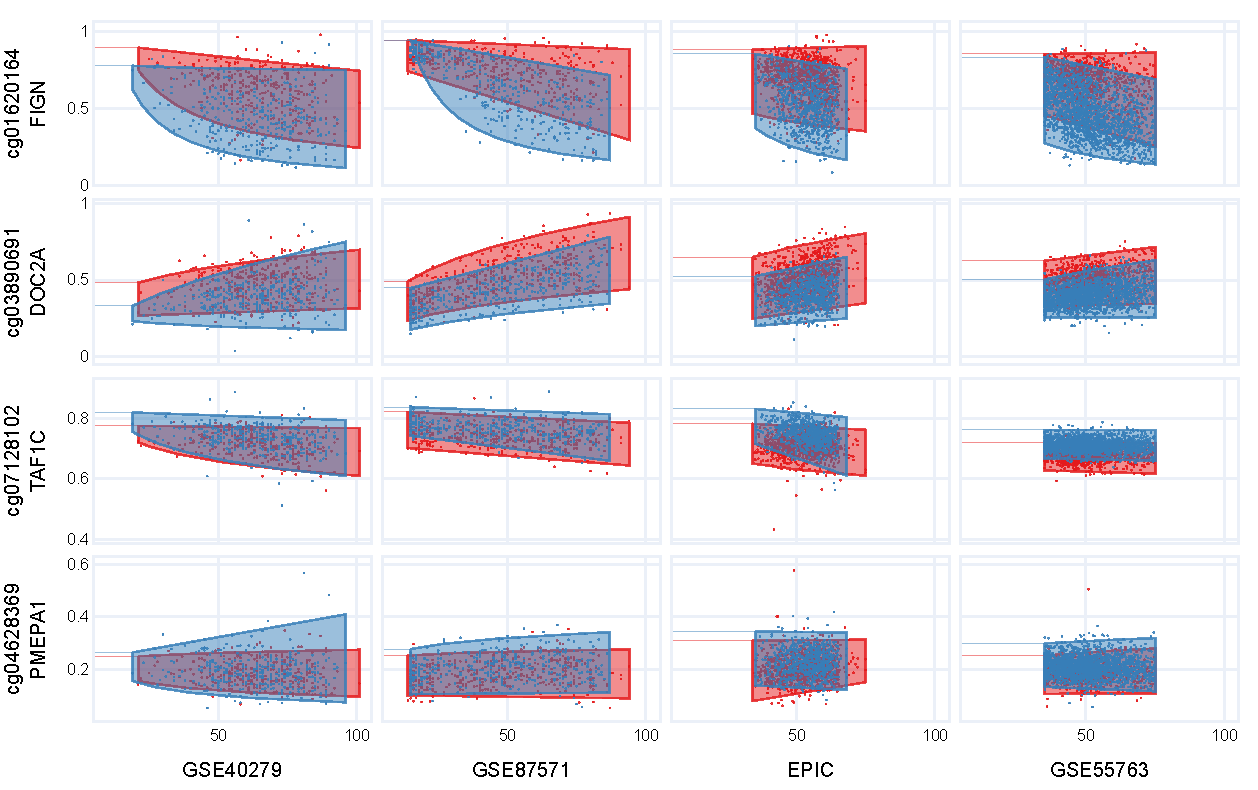
\includegraphics[scale=0.5]{saDMP.pdf}
	}
	\caption{Диаграммы разброса отдельных saDMP в рассматриваемых наборах данных.}\label{fig:saDMP_synopsis}
\end{figure}

Вторым предлагается алгоритм решения задачи поиска сайтов CpG, демонстрирующих одновременно и различия в вариабельности уровней метилирования ДНК между двумя полами, и возрастные изменения вариабельности уровня метилирования ДНК (поиск связанных с полом и возрастом различно вариабельных метилированных позиций, saVMP). Сначала каждый набор данных разделяется на два подмножества --- женщины и мужчины отдельно. Для каждого из подмножеств проводится проверка уровней метилирования на гетероскедастичность относительно возраста. Для этого используется тест Бройша-Пагана, также вычисляются соответствующие p-значения. К полученному списку p-значений применяется алгоритм METAL для выполнения взвешенного по размеру выборки метаанализа отдельно для каждого подмножества. Для полученных с помощью метаанализа p-значений проводится поправка на множественную проверку гипотез согласно алгоритму Бонферрони. Описываются 3 основных сценария половых различий в возрастной вариабельности уровней метилирования ДНК.

К рассматриваемым большим наборам данных метилирования цельной крови был применён описанный алгоритм. Было выявлено 809 и 12178 проб CpG, имеющих специфичные паттерны вариабельности для женщин и мужчин соответственно (saVMP), примеры представлены на Рисунке~\ref{fig:saVMP_synopsis}. Все специфичные для женщин saVMP показали увеличение вариабельности с возрастом, только 5 из 12178 специфичных для мужчин saVMP имеют уменьшение вариабельности уровня метилирования с возрастом. Не было выявлено ни одной пробы CpG с противоположными тенденциями изменения вариабельности уровня метилирования у обоих полов. 

\begin{figure}[ht]
	\centerfloat{
		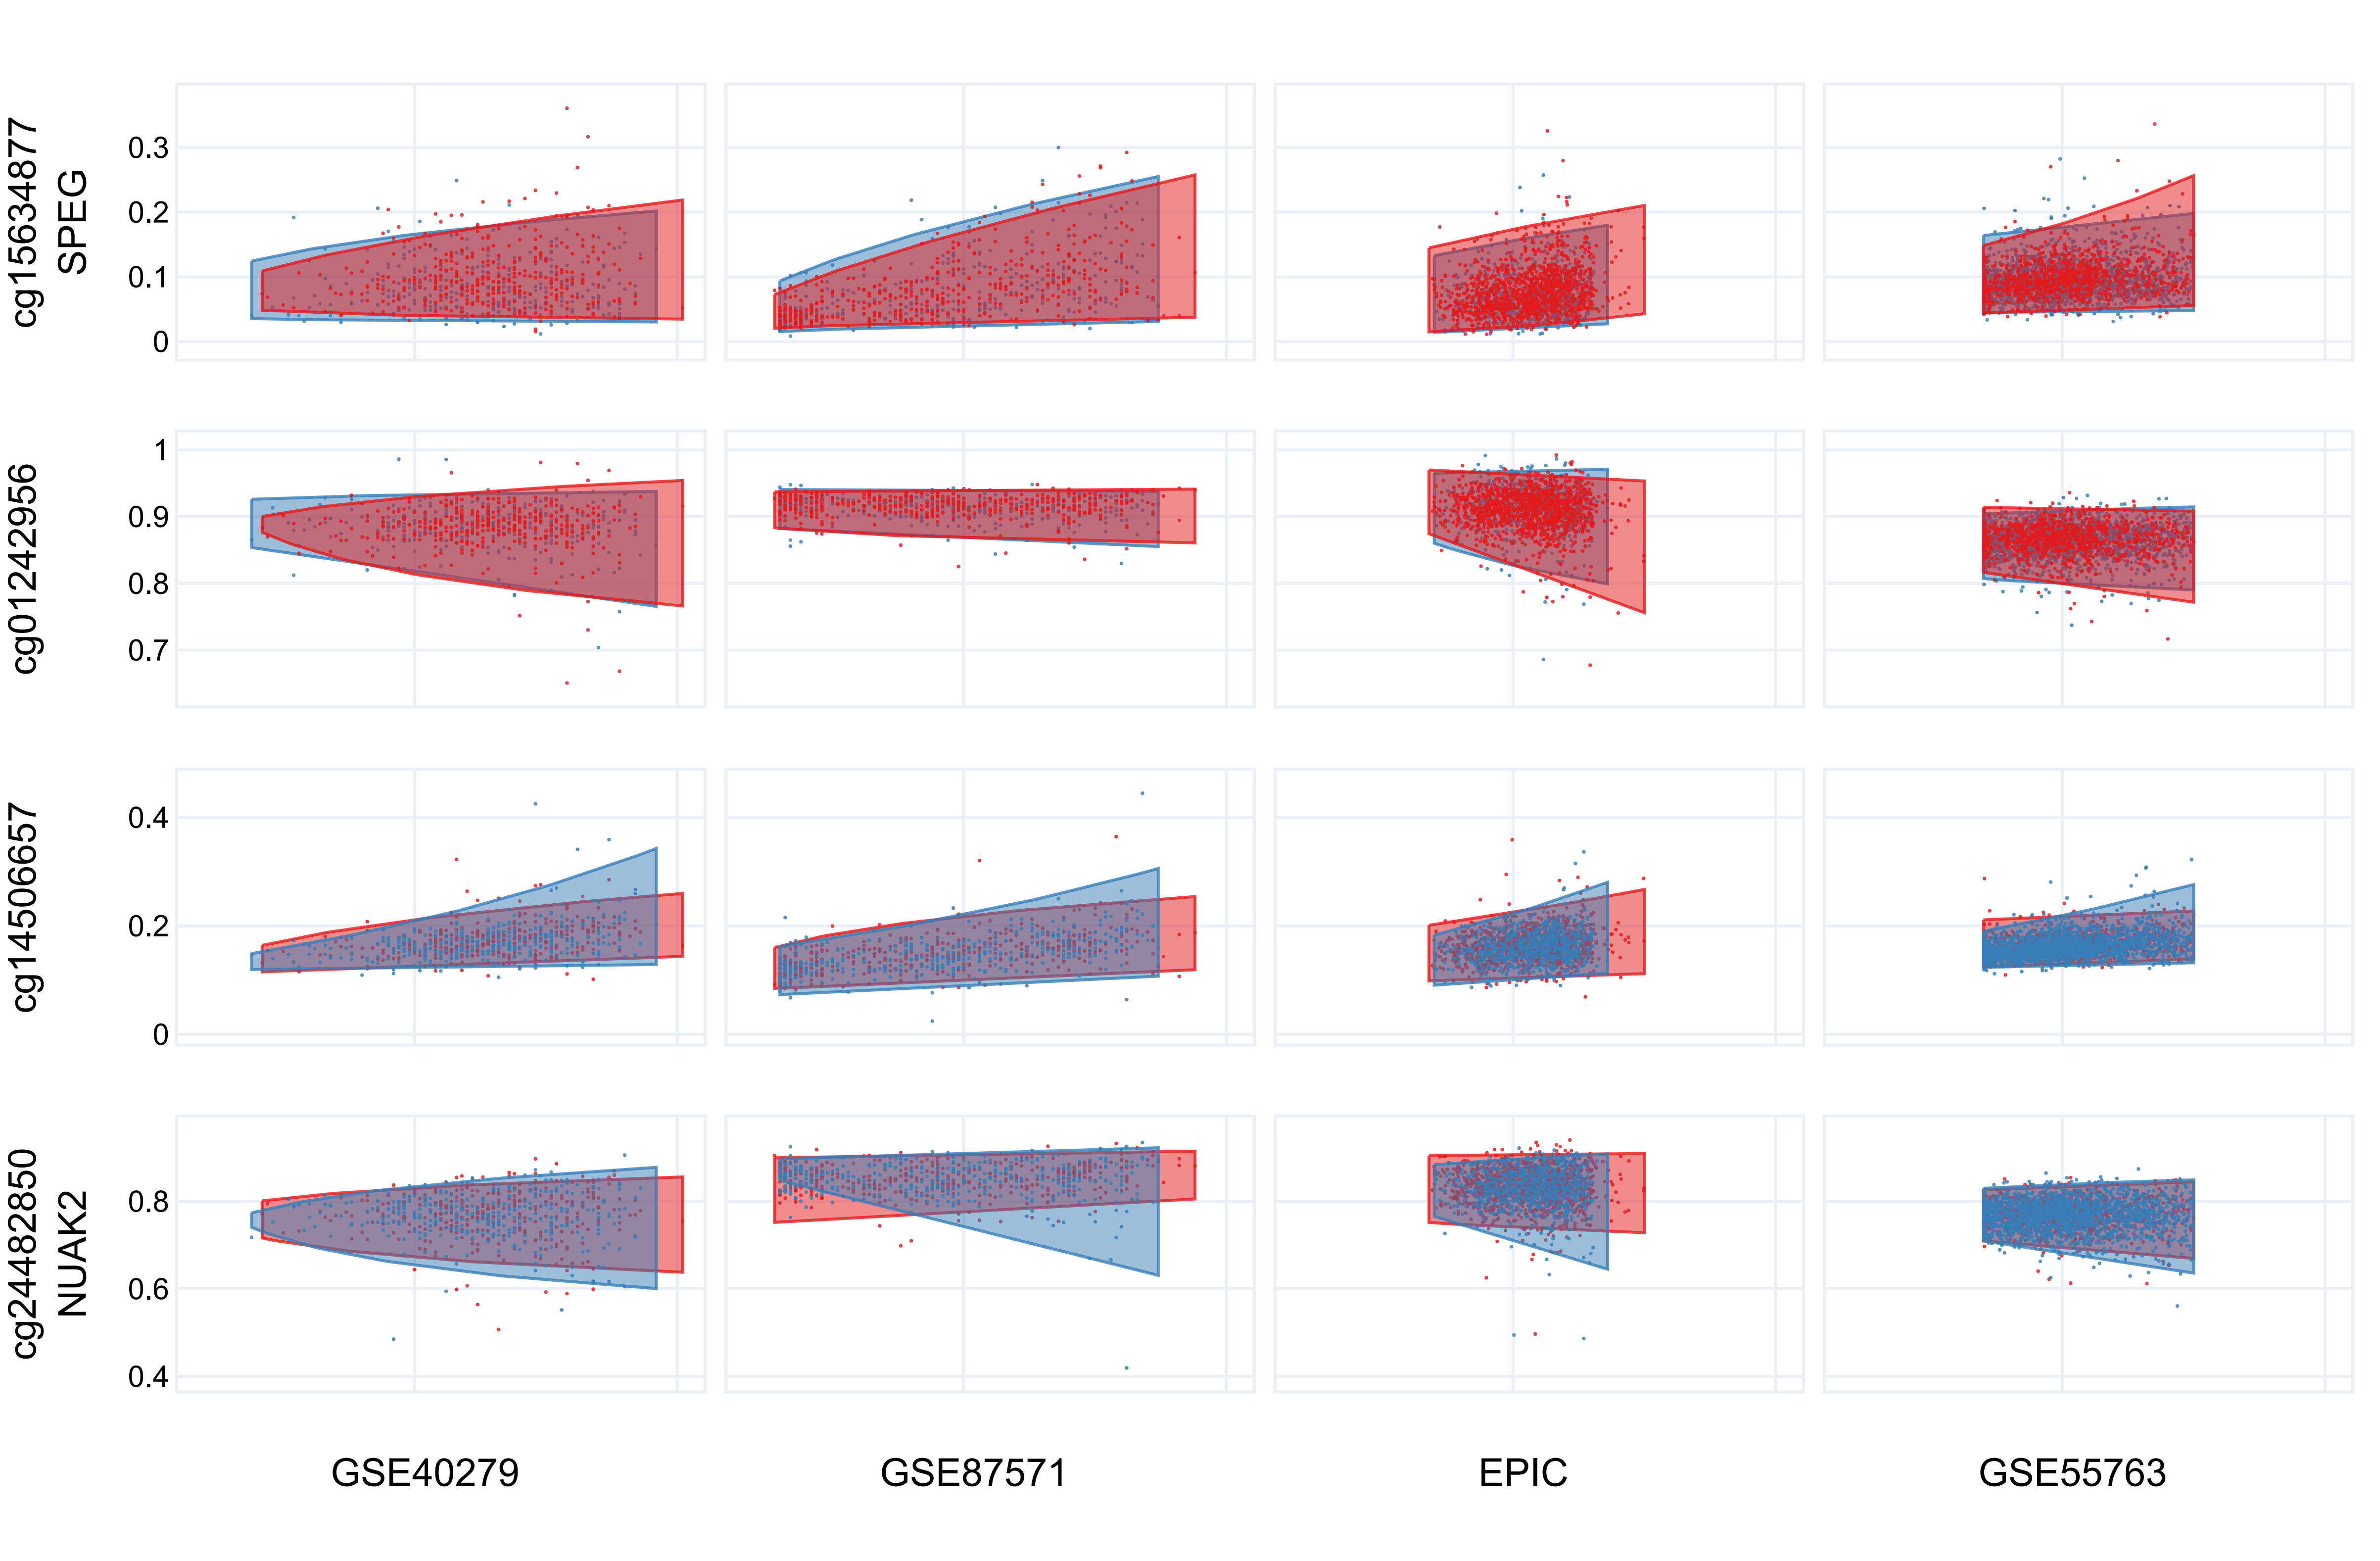
\includegraphics[scale=0.09]{saVMP.png}
	}
	\caption{Диаграммы разброса отдельных saVMP в четырёх рассматриваемых наборах данных.}\label{fig:saVMP_synopsis}
\end{figure}

В \textbf{третьей главе} описывается метод анализа генетических данных для оценки региональных различий адаптации к климатическим условиям. Входом для описываемых методов является информация об однонуклеотидных полиморфизмах митохондриальной и ядерной ДНК представителей различных популяций. Поскольку исходное количество пар митохондриально-ядерных однонуклеотидных полиморфизмов чрезмерно велико (более $10^{10}$), был разработан метод для уменьшения размерности входных данных. Рассматривается три основных типа экспериментов в зависимости от значений, принимаемыми однонуклеотидными полиморфизмами --- митохондриальная ДНК (2 варианта), ядерная ДНК (3 варианта), митохондриально-ядерные взаимодействия ДНК (6 вариантов). Для митохондриальной ДНК исключаются из рассмотрения такие однонуклеотидные полиморфизмы, которые не меняются среди всех рассматриваемых популяций --- они не несут популяционно-специфической информации. Одна из рассматриваемых популяций фиксируется как референсная. Для неё для каждого из митохондриальных генов вычисляется частота наблюдения каждого из вариантов SNP. Для каждого субъекта во всех рассматриваемых популяциях вычисляется частотная метрика каждого гена как среднее расстояние до референсной популяции. Количество вариаций для каждого из рассматриваемых субъектов будет равно количеству митохондриальных генов. Аналогично рассматривается ядерная ДНК, однонуклеотидные полиморфизмы в которой имеют один из трёх вариантов, и общий случай взаимодействия митохондриальной и ядерной ДНК. При этом пары однонуклеотидных полиморфизмов имеют один из шести парных вариантов, где первый элемент исходит от митохондриальной ДНК, второй --- от ядерной ДНК. Количество вариаций для каждого из рассматриваемых субъектов равно количеству пар взаимодействий митохондриальных и ядерных генов. Далее приводится алгоритм для определения митохондриально-ядерных взаимодействий, специфичных для популяций, проживающих в конкретных географических регионах и связанных с адаптацией к определённым климатическим условиям. Все полученные после понижения размерности частотности представим как входные переменные для алгоритма случайного леса. Данный алгоритм используется для построения и исследования моделей бинарной классификации всех пар рассматриваемых популяций. Для каждой митохондриально-ядерной пары генов, используемой в качестве входной переменной случайного леса, получим значения важности для бинарной классификации каждой пары популяций. Используя ранжированные по важности классификации списки пар генов, построим последовательные модели бинарной классификации с помощью алгоритма случайного леса с увеличивающимся числом признаков. С помощью распределений зависимости точности лкассификации от количества признаков определим оптимальную точность классификации. Каждой паре популяций присвоим список пар генов, соответствующих оптимальной точности классификации. Определим пару генов как популяционно-специфичную, если она присутствует во всех результирующих списках для данной популяции.

На примере классификации трёх популяций европейского региона показывается, что для всех пар популяций комбинации митохондриальной и ядерной ДНК показали лучшие результаты, чем классификации на основе одной мтДНК или яДНК (Таблица~\ref{tab:accuracy_synopsis}). 

\begin{table} [htbp]
	\centering
	\begin{threeparttable}
		\caption{Точность классификации для рассматриваемых популяций}%
		\label{tab:accuracy_synopsis}%
		\begin{SingleSpace}
			\begin{tabular}{| c | c | c | c |}
				\hline
				& GBR & FIN & TSI \\ \hline
				GBR      & & \thead{мтДНК: 66.84 (10) \\ яДНК: 64.21 (7) \\ мт-яДНК: 73.15 (17)}&\thead{мтДНК: 61.28 (12) \\ яДНК: 59.57 (7) \\ мт-яДНК: 70.18 (18)}\\ \hline
				FIN      & \thead{мтДНК: 66.84 (13) \\ яДНК: 66.31 (7) \\ мт-яДНК: 72.10 (19)}& &\thead{мтДНК: 75.23 (11) \\ яДНК: 75.71 (13) \\ мт-яДНК: 75.76 (69)} \\ \hline
				TSI      & \thead{мтДНК: 61.31 (13) \\ яДНК: 60.78 (9) \\ мт-яДНК: 69.28 (12)}& \thead{мтДНК: 74.78 (10) \\ яДНК: 75.69 (12) \\ мт-яДНК: 75.80 (62)}& \\ \hline
			\end{tabular}%
		\end{SingleSpace}
	\end{threeparttable}
\end{table}

Общие признаки, используемые различными классификаторами для каждой популяции, дают списки генов, частотные оценки которых на основе SNP отделяют популяцию от других. Такие популяционно-специфические гены, определяемые для различных типов экспериментов (т.е. мтДНК, яДНК, мтДНК-яДНК), перечислены в Таблице~\ref{tab:pop_specific_synopsis}.

\begin{table} [htbp]
	\centering
	\begin{threeparttable}
		\caption{Популяционно-специфичные гены, обнаруженные предложенным алгоритмом}%
		\label{tab:pop_specific_synopsis}%
		\begin{SingleSpace}
			\begin{tabular}{| c | c | c |}
				\hline
				GBR & FIN & TSI \\ \hline
				\multicolumn{3}{|c|}{Митохондриальная ДНК}\\ \hline
				\thead{MT-ATP6, MT-ND5, \\ MT-CYB, MT-CO1, \\ MT-CO3, MT-ND3, \\ MT-ND2, MT-ND1, \\ MT-ND6, MT-ND4}& \thead{MT-ATP6, MT-ND5, \\ MT-CYB, MT-CO1, \\ MT-CO3, MT-ND3, \\ MT-ND2, MT-ND1, \\ MT-ND6, MT-ND4} & \thead{MT-ATP6, MT-ND5, \\ MT-CYB, MT-CO1, \\ MT-CO3, MT-ND3, \\ MT-ND2, MT-ND1, \\ MT-ND6, MT-ND4}\\ \hline
				\multicolumn{3}{|c|}{Ядерная ДНК}\\ \hline
				PDRM16, LEPR, DIO2 & \thead{PDRM16, LEPR, DIO2, \\ PPARG, NRF1} & \thead{PDRM16, LEPR, DIO2, \\ UCP3, CIDEA, PLIN1} \\ \hline
				\multicolumn{3}{|c|}{Митохондриально-ядерная ДНК}\\ \hline
				& \thead{MT-CYB+FTO, \\ MT-ND2+HOXA1, \\ MT-CYB+PRDM16, \\ MT-ND5+NRF1, \\ MT-CYB+DIO2, \\ MT-ND1+NRF1, \\ MT-CYB+HOXA1, \\ MT-ND3+NRF1, \\ MT-ND1+HOXA1, \\ MT-CYB+NRF1}& \thead{MT-ATP6+PRDM16, \\ MT-CYB+UCP2, \\ MT-ND1+CIDEA, \\ MT-ND3+DIO2, \\ MT-RNR1+DIO2, \\ MT-CO3+LEPR, \\ MT-ATP6+UCP2, \\ MT-ND2+CIDEA, \\ MT-RNR1+CIDEA, \\ MT-ND4+DIO2}\\ \hline
			\end{tabular}%
		\end{SingleSpace}
	\end{threeparttable}
\end{table}


\FloatBarrier
\pdfbookmark{Заключение}{conclusion}                                  % Закладка pdf
В \textbf{заключении} приведены основные результаты работы, которые заключаются в следующем:
%% Согласно ГОСТ Р 7.0.11-2011:
%% 5.3.3 В заключении диссертации излагают итоги выполненного исследования, рекомендации, перспективы дальнейшей разработки темы.
%% 9.2.3 В заключении автореферата диссертации излагают итоги данного исследования, рекомендации и перспективы дальнейшей разработки темы.
\begin{enumerate}
  \item Разработан метод поиска связанных с возрастом специфичных для пола биомаркеров, включающий также раздельный поиск связанных с возрастом и специфичных для пола биомаркеров. Он основан на проведение корреляционного анализа и метаанализа множества наборов данных.
  \item Разработан алгоритм поиска биомаркеров с возрастной вариабельностью, связанной с полом, предполагающий тестирование на гетероскедастичность и проведение метаанализа множества наборов данных. Описаны основные сценарии поведения половых различий в возрастной вариабельности уровня метилирования ДНК.
  \item Разработан программный комплекс, реализующий указанные методы и позволяющий осуществлять полный цикл работы алгоритма от обработки входных данных до вывода результирующих биомаркеров и визуализации. Метод доступен для использования в виде программного пакета для языка Python в репозитории Python Package Index (https://pypi.org/project/pydnameth).
  \item Разработан метод поиска митохондриально-ядерных взаимодействий, специфичных для популяций, проживающих в определённых климатических условиях. Он основан на построении серии последовательных моделей случайного леса с увеличивающимся количеством признаков. Кроме того, ввиду большой размерности входных данных, разработан алгоритм её сокращения путём усреднения информации о генетических вариациях внутри каждого гена.
  \item Разработан программный комплекс, реализующий указанные алгоритмы и позволяющий осуществлять полный цикл работы алгоритма: обработка входных данных, уменьшение размерности входных данных, реализация алгоритма, получение результатов.
  \item Для всех разработанных методов проведена экспериментальная проверка работоспособности на реальных биологических данных, показана корректность получаемых результатов, приведено обоснование с биологической точки зрения.
\end{enumerate}


\pdfbookmark{Литература}{bibliography}                                % Закладка pdf

\ifdefmacro{\microtypesetup}{\microtypesetup{protrusion=false}}{} % не рекомендуется применять пакет микротипографики к автоматически генерируемому списку литературы
\urlstyle{rm}                               % ссылки URL обычным шрифтом
\ifnumequal{\value{bibliosel}}{0}{% Встроенная реализация с загрузкой файла через движок bibtex8
  \renewcommand{\bibname}{\large \bibtitleauthor}
  \nocite{*}
  \insertbiblioauthor           % Подключаем Bib-базы
  %\insertbiblioexternal   % !!! bibtex не умеет работать с несколькими библиографиями !!!
}{% Реализация пакетом biblatex через движок biber
  % Цитирования.
  %  * Порядок перечисления определяет порядок в библиографии (только внутри подраздела, если `\insertbiblioauthorgrouped`).
  %  * Если не соблюдать порядок "как для \printbibliography", нумерация в `\insertbiblioauthor` будет кривой.
  %  * Если цитировать каждый источник отдельной командой --- найти некоторые ошибки будет проще.
  %
  %% authorprogram
  \nocite{prog1}%
  %
  %% authorconf
  \nocite{conf1}%
  \nocite{conf2}%
  \nocite{conf3}%
  \nocite{conf4}%

  \ifnumgreater{\value{usefootcite}}{0}{
    \begin{refcontext}[labelprefix={}]
      \ifnum \value{bibgrouped}>0
        \insertbiblioauthorgrouped    % Вывод всех работ автора, сгруппированных по источникам
      \else
        \insertbiblioauthor      % Вывод всех работ автора
      \fi
    \end{refcontext}
  }{
  \ifnum \totvalue{citeexternal}>0
    \begin{refcontext}[labelprefix=A]
      \ifnum \value{bibgrouped}>0
        \insertbiblioauthorgrouped    % Вывод всех работ автора, сгруппированных по источникам
      \else
        \insertbiblioauthor      % Вывод всех работ автора
      \fi
    \end{refcontext}
  \else
    \ifnum \value{bibgrouped}>0
      \insertbiblioauthorgrouped    % Вывод всех работ автора, сгруппированных по источникам
    \else
      \insertbiblioauthor      % Вывод всех работ автора
    \fi
  \fi
  %  \insertbiblioauthorimportant  % Вывод наиболее значимых работ автора (определяется в файле characteristic во второй section)
  \begin{refcontext}[labelprefix={}]
      \insertbiblioexternal            % Вывод списка литературы, на которую ссылались в тексте автореферата
  \end{refcontext}
  % Невидимый библиографический список для подсчёта количества внешних публикаций
  % Используется, чтобы убрать приставку "А" у работ автора, если в автореферате нет
  % цитирований внешних источников.
  \printbibliography[heading=nobibheading, section=0, env=countexternal, keyword=biblioexternal, resetnumbers=true]%
  }
}
\ifdefmacro{\microtypesetup}{\microtypesetup{protrusion=true}}{}
\urlstyle{tt}                               % возвращаем установки шрифта ссылок URL
